%!TEX root = ../Thesis.tex
\paragraph{}
The steady growth of fitness and health conscious consumers has urged many companies to take note of wearables industry. The shipments of global wearable devices are expected to grow 55\% by 2022.\cite{WearableStudy} Most of which are expected to be smart-watches and wrist-worn fitness trackers. To lure the consumer companies are urged to innovate. Enabling consumers to monitor their personal health more closely.
\begin{figure}
	\centering
	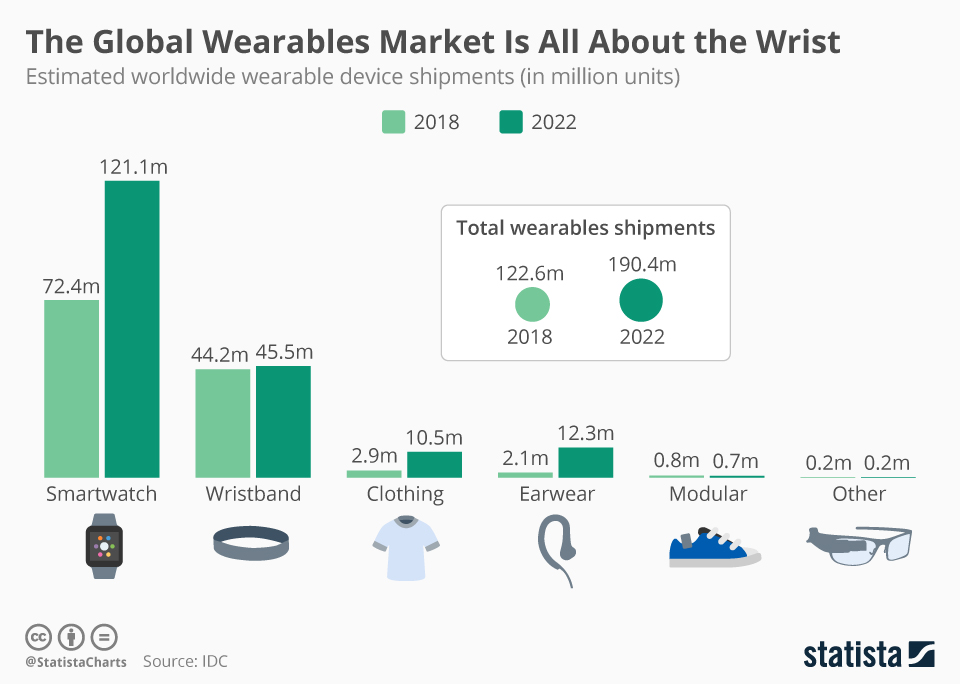
\includegraphics[width=100mm]{wearable_device_forecast.jpg}
	\caption{Forecast of Wearable Devices 2018-2022}
	\label{fig:forecast_of_wearable_devices}
\end{figure}
\paragraph{}
Apple introduced Electrocardiogram (ECG) feature in Apple Watch Series 4 on September 12, 2018. It is evident that companies are now looking beyond fitness tracking by enabling users to monitor their health with consumer end wearable devices, which was once only possible with high-end medical devices.
\paragraph{}
The inception of health monitoring is sure to open new avenues in recording more complex physiological information with higher accuracy. A study conducted by C. McCarthy et. al. found that the Empatica's E4 portable Photoplethysmogram (PPG) almost on par with the clinician standard device for atrial fibrillation diagnosis. \cite{7508621}
\paragraph{}
Vivid physiological signals like Electrocardiogram (ECG), Electrodermal Activity (EDA), Photoplethysmogram (PPG), Skin Temperature, Blood Pressure etc. in consumer grade wearable devices enables availability of instant health data. While this has enormous health benefits, it also raises several privacy concerns.
\paragraph{}
The wearable devices connect to several mobile application which provide for easy monitoring of physiological data. As the users of the wearable devices and mobile applications the consumers are often contributing to centralized database maintained by these companies. While advertising, “we respect your privacy”. The privacy policies of the companies are often misguided with confusing wordings like “we \textit{may} share your information with third party providers.”
\paragraph{}
The consequences of such critical data being handed over to companies are far reaching. In 2011, Fitbit was heavily criticized for tracking user’s sexual activity and making it available over the user’s public profile on its online platform which could be easily found with a simple Google search.\cite{Fitbit} Fitbit was able to determine user’s sexual activity using accelerometer in the devices. The physiological information is way more personal.
This begs for a very important question. What can be determined about the user’s activity and psychological state with availability of physiological information.
\paragraph{}
In this thesis we try to determine if we can predict viewing activity of a user based on their physiological data. We consider Electrocardiogram (ECG) and Electrodermal Activity (EDA) as determiner. We took into consideration 10 short movies ranging from three minutes to twelve minutes, spread across comedy, horror, romantic, thriller and action movies. We collected data of 20 subjects for each movie of which 17 were used to train the data and 3 were used to test our model. 